\documentclass[a4paper,11pt]{article}
\usepackage{jcappub}
\usepackage[T1]{fontenc}
\usepackage{booktabs,xcolor,orcidlink,placeins}
\hypersetup{colorlinks=true, linkcolor=blue!55!black, citecolor=blue!55!black, urlcolor=blue!55!black}
\newcommand{\lcdm}{\ensuremath{\Lambda\mathrm{CDM}}}
\newcommand{\wz}{\ensuremath{w_0}}
\newcommand{\wa}{\ensuremath{w_a}}
% GENERATED by pipeline/gen_paper_numbers.py -- do not edit.
% Sources: runs/phase3/fparam/ah.json, runs/gate2/gate2_final_stats.json, runs/prd_extension/null500/endpoints.json, runs/prd_extension/wp3_power/power_report.json, runs/phase2/fate/d0_cpl_p1.json, runs/phase3/fparam/{prior_fate_audit,fate_*,model_average_audit}.json
\newcommand{\KLbinA}{3.03}
\newcommand{\KLbinB}{2.31}
\newcommand{\KLbinC}{1.55}
\newcommand{\KLbinD}{0.24}
\newcommand{\NullAcc}{50}
\newcommand{\NullKSp}{0.25}
\newcommand{\NullMean}{0.525}
\newcommand{\NullMeanSE}{0.030}
\newcommand{\RipNullMin}{1.52}
\newcommand{\NullFiveN}{500}
\newcommand{\NullFiveK}{2}
\newcommand{\NullFiveTailPct}{0.40}
\newcommand{\NullFivePlusOne}{0.00599}
\newcommand{\NullFiveCPLow}{0.000485}
\newcommand{\NullFiveCPHigh}{0.0144}
\newcommand{\NullFiveDirectionK}{264}
\newcommand{\NullFiveDirectionPct}{52.8}
\newcommand{\NullFiveDirectionLowPct}{48.3}
\newcommand{\NullFiveDirectionHighPct}{57.2}
\newcommand{\NullFiveKSp}{0.154}
\newcommand{\NullFiveRipMinPct}{0.166}
\newcommand{\NullFiveOtherMaxPct}{0.254}
\newcommand{\NullFiveBoundaryMaxPct}{0.139}
\newcommand{\DzeroDecayPct}{99.82}
\newcommand{\DzeroRipPct}{0.18}
\newcommand{\DzeroRipErrPct}{0.06}
\newcommand{\NestedDzeroRipPct}{0.179}
\newcommand{\NestedDzeroRipSeedSdPct}{0.039}
\newcommand{\NestedDzeroRipMinPct}{0.135}
\newcommand{\NestedDzeroRipMaxPct}{0.209}
\newcommand{\NestedDzeroOtherPct}{0.0093}
\newcommand{\NestedLnB}{-1.617}
\newcommand{\NestedLnBSeedSd}{0.224}
\newcommand{\NestedLnBMin}{-1.865}
\newcommand{\NestedLnBMax}{-1.431}
\newcommand{\NestedLnBInternalMin}{0.313}
\newcommand{\NestedLnBInternalMax}{0.314}
\newcommand{\ModelAvgLCDMPct}{83.4}
\newcommand{\ModelAvgCPLPct}{16.6}
\newcommand{\ModelAvgHeatPct}{99.97}
\newcommand{\DOneNestedRipPct}{0.376}
\newcommand{\DTwoNestedRipPct}{0.067}
\newcommand{\DThreeNestedRipPct}{0.0008}
\newcommand{\DFourNestedRipPct}{0.189}
\newcommand{\FDataNestedRipMinPct}{0.0008}
\newcommand{\FDataNestedRipMaxPct}{0.376}
\newcommand{\GrammarRipMinPct}{0.21}
\newcommand{\GrammarRipMaxPct}{49.96}
\newcommand{\GrammarHeatMinPct}{50.04}
\newcommand{\GrammarHeatMaxPct}{99.79}
\newcommand{\PriorRipMinPct}{25.8}
\newcommand{\PriorRipMaxPct}{58.4}
\newcommand{\BAPriorRipPct}{58.4}
\newcommand{\BINPriorRipPct}{50.6}
\newcommand{\BARipPct}{1.34}
\newcommand{\BADecayPct}{98.66}
\newcommand{\BABoundaryPct}{0.35}
\newcommand{\BINRipPct}{49.96}
\newcommand{\BINDecayPct}{50.04}
\newcommand{\BINBoundaryPct}{17.6}
\newcommand{\FPriorRip}{\infty}
\newcommand{\FPriorHeat}{0.002}
\newcommand{\FParamRip}{\infty}
\newcommand{\FParamHeat}{0.301}
\newcommand{\FParamFitsRip}{2.380}
\newcommand{\FParamFitsHeat}{0.300}
\newcommand{\FDataRip}{2.665}
\newcommand{\FDataHeat}{0.002}
\newcommand{\RCPL}{0.0063}
\newcommand{\RJBP}{0.0093}
\newcommand{\RBA}{0.0026}
\newcommand{\RBIN}{0.0046}
\newcommand{\WpWamSixtyDeltaChi}{0.00}
\newcommand{\WpWamSixtyDirection}{1.00 [0.964,1.000]}
\newcommand{\WpWamSixtyDepth}{0.90 [0.824,0.951]}
\newcommand{\WpWamSixtyFalse}{0.00 [0.000,0.036]}
\newcommand{\WpWamThirtyDeltaChi}{1.67}
\newcommand{\WpWamThirtyDirection}{0.93 [0.861,0.971]}
\newcommand{\WpWamThirtyDepth}{0.47 [0.369,0.572]}
\newcommand{\WpWamThirtyFalse}{0.07 [0.029,0.139]}
\newcommand{\WpWamFifteenDeltaChi}{4.05}
\newcommand{\WpWamFifteenDirection}{0.84 [0.753,0.906]}
\newcommand{\WpWamFifteenDepth}{0.33 [0.239,0.431]}
\newcommand{\WpWamFifteenFalse}{0.16 [0.094,0.247]}
\newcommand{\WpWapFifteenDeltaChi}{12.71}
\newcommand{\WpWapFifteenDirection}{0.77 [0.675,0.848]}
\newcommand{\WpWapFifteenDepth}{0.18 [0.110,0.269]}
\newcommand{\WpWapFifteenFalse}{0.23 [0.152,0.325]}
\newcommand{\WpWapThirtyDeltaChi}{19.45}
\newcommand{\WpWapThirtyDirection}{0.93 [0.861,0.971]}
\newcommand{\WpWapThirtyDepth}{0.57 [0.467,0.669]}
\newcommand{\WpWapThirtyFalse}{0.07 [0.029,0.139]}
\newcommand{\WpWapSixtyDeltaChi}{39.37}
\newcommand{\WpWapSixtyDirection}{1.00 [0.964,1.000]}
\newcommand{\WpWapSixtyDepth}{0.98 [0.930,0.998]}
\newcommand{\WpWapSixtyFalse}{0.00 [0.000,0.036]}
 % GENERATED from runs/ JSON by pipeline/gen_paper_numbers.py

\title{\boldmath Is cosmic fate an inference or an assumption?\texorpdfstring{\\}{: }
A locally preregistered fragility audit of cosmic-fate inference\texorpdfstring{\\}{ }
with DESI DR2, Pantheon+, and \textit{Planck}}

\author[a]{Jiacheng Zhang\,\orcidlink{0009-0007-7438-320X}}
\affiliation[a]{Independent researcher}
\emailAdd{shlinawaf717@gmail.com}

\abstract{
The DESI era has renewed interest in the ultimate fate of the Universe. We ask
how much of a fate verdict is constrained by data and how much is induced by
assumptions. We combine DESI DR2 BAO, \textit{Planck} 2018 distance priors,
and Pantheon+/SH0ES supernovae under a locally preregistered analysis plan,
propagate posterior samples through a frozen fate classifier, calibrate the
verdict with repeated data, and vary its prior, statistic, parametrization,
and future-continuation rule. Within CPL and the baseline prior, the posterior
Big Rip probability is \DzeroRipPct\%, with a nested-sampling point estimate
of \NestedDzeroRipPct\%. Across \NullFiveN{} fitted-truth \lcdm{} mocks, the
heat-death-compatible posterior mass is consistent with a uniform
distribution; \NullFiveK{} mocks are at least as deep in the anti-rip tail as
the data, giving a plus-one estimate of \NullFivePlusOne{} with an exact 95\%
interval of \NullFiveCPLow{}--\NullFiveCPHigh. A quintessence prior excludes
the rip before data are considered. Four converged native-prior
parametrizations yield Big Rip probabilities from \GrammarRipMinPct\% to
\GrammarRipMaxPct\%, while their induced prior rip masses already span
\PriorRipMinPct\%--\PriorRipMaxPct\%. This is a sensitivity audit, not a
common-prior model comparison: the four pushforwards occupy incompatible
supports in function space. A calibrated seven-node reconstruction leaves its
final future node essentially prior-dominated. Holding the entire history up
to the present, all current-background observables, and the likelihood fixed,
four registered continuation families give a descriptive Big Rip envelope of
\WPEightEnvelopeRipMinPct\%--\WPEightEnvelopeRipMaxPct\%;
\WPEightTwoSidedPct\% of source-history weight admits both rip and
heat-death-compatible continuations. These kinematic continuations are not
asserted to be stable covariant microphysical theories, and no probability is
assigned to them. Current observations can therefore yield sharp fate
probabilities within an adopted model, but do not identify a unique infinite
future without a physical continuation law. All quantitative results are
background-level and conditional on the compressed-CMB likelihood.
}

\keywords{dark energy theory; Bayesian reasoning; statistical sampling
techniques; baryon acoustic oscillations}

\begin{document}
\maketitle
\flushbottom

\section{Introduction}\label{sec:intro}

The DESI era has revived the oldest question in cosmology. Baryon acoustic
oscillation measurements from DESI DR2, combined with cosmic microwave
background (CMB) and Type Ia supernova data, favor solutions in the
``thawing'' quadrant $\wz>-1$, $\wa<0$ \cite{DESIDR2}. The reported strength
is analysis-dependent. The original official combinations gave
$2.8$--$4.2\sigma$; subsequent supernova recalibration brings corrected
Pantheon+, Union3.1, and DES-Dovekie combinations into the narrower
$3.2$--$3.4\sigma$ range, while fully Bayesian evidence calculations can
modestly favor \lcdm{} after the extended model's prior volume is included
\cite{DESIDR2,Dovekie2025,Union31,BayesianDESIDR2,
CompressedEvidence2025,Efstathiou2024,HuangCaiWang2025,WangMota2025}.
After this analysis freeze, DESI added a one-percent Alcock--Paczy\'nski
measurement from the same DR2 Ly$\alpha$ forest used for its BAO point. The
joint Ly$\alpha$ AP+BAO update reports $2.7\sigma$ for DESI+CMB and
$3.2\sigma$ after adding supernovae, slightly reducing rather than eliminating
the dynamical-dark-energy discrepancy \cite{DESIDR2ResultsIV}.
Specific parametrizations and physical models have long been translated into
future-fate statements, including work designed explicitly to avoid CPL's
unbounded future behavior
\cite{LiFate2012,AndreiIjjasSteinhardt2022,Gialamas2025}.

This paper asks a different question. Rather than ``what is the fate?'', we
ask: \emph{of the fate verdict, how much is forced by the data, and how much
is donated by the assumptions?} The question has a distinguished qualitative
pedigree---Krauss and Turner~\cite{KraussTurner1999} argued a quarter-century ago that dark
energy severs the link between geometry and destiny, and
Kallosh and Linde~\cite{KalloshLinde2003} computed observational doomsday bounds for specific
potentials. We are unaware of a published study that combines an end-to-end
repeated-\lcdm{}-mock calibration of a posterior fate-class probability with a
finite sensitivity audit over the eight analysis axes declared here. This is
the paper's scoped methodological contribution, not a claim that earlier work
ignored model dependence.

The paper separates three questions. First, within a specified CPL analysis,
what fate probability is obtained and how does that statistic behave under
repeated \lcdm{} data? Second, how does the verdict respond to data choices,
priors, inference statistics, and four commonly used parametrizations? Third,
after the entire observed history is fixed, what remains unidentified about
its continuation? This ordering separates a model-conditional numerical
result from the broader question of whether present data license an infinite-
future extrapolation.

Three results organize the answer. Within continuous CPL, the direction-class
posterior mass is consistent with $U(0,1)$ when the truth is exactly on the
\lcdm{} fate boundary, while the real data lie unusually deep in its anti-rip
tail. Across native-prior parametrizations, similar descriptive in-window fit
quality coexists with posterior Big Rip probabilities from approximately
$0.2\%$ to $50\%$; these are complete-analysis sensitivity diagnostics rather
than a common-prior model competition. Finally, a calibrated seven-node fit
and an exact fixed-history continuation audit show that apparent future-node
information can be transported by prior correlations and that the registered
continuations of one observed history support both thermodynamic sides. The
last statement is a partial-identification result within a declared kinematic
class, not an impossibility theorem for all microphysical theories.

We therefore report current fate estimates as model-conditional predictions
whose structural uncertainty is not contained in their within-model posterior
intervals. The contribution is a locally preregistered, repeated-data-
calibrated sensitivity protocol that makes the conditioning explicit.

\section{Preregistered inference framework}\label{sec:prereg}

The analysis plan specified the model space, priors, dataset combinations,
criteria for classifying fates, statistical rules, and pass/fail gates. The
protocol was written and frozen in local version control before the first
target fate calculation, according to the preserved Git history. Because the
repository was made public only afterwards, the original freeze lacks an
independently verifiable timestamp. We therefore describe the study as locally
preregistered, not as a registry-verified preregistration. Specifically, commit
\texttt{98abc20} under tag
\texttt{prereg-v1}, recorded at 10:26 local time on 2026-07-03, is an ancestor
of the first real-data fate-result commit recorded at 11:29. The frozen plan is
reproduced in English translation in Appendix~\ref{app:plan}; commit ancestry,
timestamps, tree identifiers, and the plan checksum are listed in the archived
provenance audit, \path{plan/PREREGISTRATION_PROVENANCE.md}.

More precisely, this is a secondary-data preregistration of the fate-translation
audit. The datasets and validation strategy were already known, but the core
classifier, audit axes, gates, and two reportable outcome forms were frozen
before the first target fate calculation. It is not a claim of preregistration
before data access or of an independently timestamped public registration.

The 500-mock, off-boundary-power, seven-node, and fixed-history continuation
results were not part of the original local preregistration. They belong to a
separately versioned strengthening protocol, frozen before the corresponding
results. The immutable historical checkpoint is tag
\texttt{paper-v1x-final-20260722}; extension products are isolated below
\path{runs/prd_extension/}. We describe this layer as a prospectively
specified public extension, not as part of the original preregistered core.
Its append-only ledger records execution-order deviations and corrective
scope changes.

Departures from the frozen plan are recorded in an append-only log
(Appendix~\ref{app:amendments}) stating what changed, why, and when relative to
data contact. Three amendments to the frozen core occurred: A-001 recalibrated
the pipeline-validation benchmark after we established that a compressed-CMB
likelihood cannot reproduce the full-likelihood exclusion significance
(Sec.~\ref{sec:data}); A-002 replaced a mock-recovery criterion that is
mathematically unsatisfiable for a truth on a fate boundary
(Sec.~\ref{sec:null}); and A-003 added an analytic fate branch after the frozen
\textsc{other}-budget audit was triggered by bounded-future parametrizations
(Sec.~\ref{sec:fparam}). In each case the trigger, argument, and sign-off are
logged. Four later records are explicitly post-hoc: A-004 tests whether the
grammar-specific priors can be matched by importance reweighting; A-005
corrects the finite-limit fate semantics without altering CPL-based results;
A-006 adds an early-dark-energy hard gate; and A-007 documents the
model-specific translation of P1's early-matter-domination intent without
retroactively treating that implementation detail as explicitly
preregistered.

The data also predate the plan: DESI DR2 constraints were public before the
freeze. The version-controlled record documents analysis-choice discipline---a
declared classifier, gates, fragility metrics, and two equally reportable
outcome forms---rather than prediction novelty. The published $\wz$--$\wa$
constraint is used only as a Gate-1 validation target. Six analytical checks
for the null campaign were recorded after approximately 17 of 100 mocks and
before the remaining campaign completed; they are prospective checks for the
remaining runs, not pre-analysis registrations. The zero-residual prediction
was recorded before that run (Appendix~\ref{app:mocks}). This discipline is
weaker than survey blinding, which can shield catalogs or data vectors from the
analyst~\cite{Muir2020,Andrade2025}; it makes the workflow auditable but does
not eliminate all analyst degrees of freedom. The methodological contribution
is the resulting transparent sensitivity audit, not an external-registry claim.

\subsection{Data, likelihoods, and validation}\label{sec:data}

We use three publicly released datasets: DESI DR2 BAO compressed measurements
(13 points over seven redshift bins, $0.295\le z\le 2.33$)~\cite{DESIDR2};
the Pantheon+ Type Ia supernova compilation with full stat+sys covariance,
with and without the SH0ES Cepheid anchor~\cite{Scolnic2022,Brout2022,Riess2022}; and \textit{Planck}
2018 information~\cite{Planck2018} compressed into the distance priors $(R,\ell_A,\Omega_b h^2)$
of Ref.~\cite{ChenHuangWang2018}, validated there for CPL-type models. Files,
versions, and checksums are registered in the repository manifest
(Appendix~\ref{app:repro}).

Two validation results define what the pipeline can claim. First, against the
official DESI DR2 $w_0w_a$CDM chains, our marginals agree to $\le0.33\sigma$
in every parameter, with $\Omega_m$ agreeing to $<0.1\sigma$ and $H_0$ to
$<0.25\sigma$
(Fig.~\ref{fig:gate1}). Second, the compressed CMB prior carries a known,
stable information deficit: our \lcdm{} exclusion is $2.25\sigma$
($\Delta\chi^2=7.44$) where the full-likelihood value is $2.8\sigma$, and the
same $\approx0.5\sigma$ discount recurs across all three supernova
compilations (Sec.~\ref{sec:fdata}), consistent with independent
compressed-likelihood analyses~\cite{CompressedEvidence2025}. Every
significance below inherits the compressed-CMB condition; we price it rather
than hide it. One procedural lesson is worth recording: compressed priors
must be predicted with the same $z_*$/$r_s$ conventions used at extraction---
mixing conventions shifted $\ell_A$ by $3\sigma$ of pure artifact in an early
pipeline version, caught by a known-answer test before any science ran.

\begin{figure}[t]
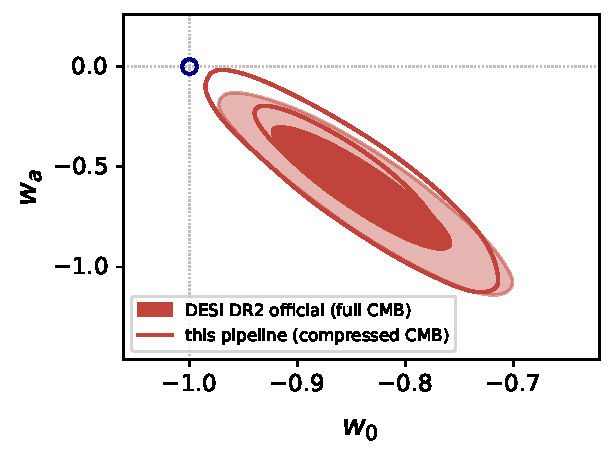
\includegraphics[width=0.9\columnwidth]{../runs/gate1/f1_gate1_vs_official.pdf}
\caption{Gate-1 chain-level validation: this pipeline (compressed CMB, open
contours) versus the official DESI DR2 chains (full CMB + lensing, filled).
All marginal shifts $\le 0.33\sigma$. Here and throughout, contour pairs
show the 68\% and 95\% credible regions.}\label{fig:gate1}
\end{figure}

\subsection{Fate taxonomy and classifier}\label{sec:fate}

Each posterior sample defines a background
\begin{equation}
\frac{H^2(a)}{H_0^2}=\Omega_r a^{-4}+\Omega_m a^{-3}
 +\Omega_k a^{-2}+\Omega_{\rm DE}f_{\rm DE}(a),
\end{equation}
integrated from $a=1$ to $a_{\max}=10^4$ and
classified with frozen criteria, in priority order: \textsc{crunch}
($H^2\le0$ reached); \textsc{rip} (finite-time singularity~\cite{Caldwell2003}: convergent
$\int\!da/aH$; for parametrizations whose $w(a)$ has a finite limit
$w_\infty$, A-003 introduced an analytic branch and A-005 corrects its
physical boundary to $w_\infty<-1$); \textsc{ds} (exact de Sitter
asymptotics, $w_\infty=-1$ with persistent dark energy, in the finite-limit
branch); \textsc{decay} (dark-energy
dilution); \textsc{other} (unclassifiable---audited under a frozen 1\% budget
whose breach triggers the amendment process, as occurred for A-003). Every
class carries a boundary flag: numerical-branch samples that flip when
thresholds are doubled or halved, and finite-limit samples satisfying
$|w_\infty+1|\le0.01$, are reported as boundary-adjacent without changing
their physical label.

For this audit, \textsc{ds} and \textsc{decay} are grouped into a coarse
heat-death-compatible macroclass because both avoid a finite-time singularity
and expand forever in the flat backgrounds considered here. This operational
grouping does not assert thermodynamic equivalence: horizon structure,
temperature floors, and accessible free energy can differ between the two.
Within flat CPL backgrounds the only non-heat-death branch is the Big Rip. The
classifier passes a ten-case unit suite spanning all classes, boundary
behavior, and two documented numerical edge cases
(Appendix~\ref{app:classifier}).

\section{Conditional fate inference in CPL}\label{sec:baseline}

Figure~\ref{fig:partition} shows the D0 (DESI DR2 + CMB prior + Pantheon+SH0ES)
CPL~\cite{ChevallierPolarski2001,Linder2003} posterior, with
\begin{align*}
\wz&=-0.884\pm0.057, & \wa&=-0.62^{+0.25}_{-0.22},\\
\Omega_m&=0.2997\pm0.0050, &
H_0&=69.00\pm0.54~\mathrm{km\,s^{-1}\,Mpc^{-1}},
\end{align*}
from four chains with $R-1=0.0033$, drawn over the fate partition of the
$(\wz,\wa)$ plane. The posterior presses
against the zero-width \textsc{rip}/\textsc{decay} boundary at $\wa=0$; the
consequences of that geometry occupy the next section.

\begin{figure}[t]
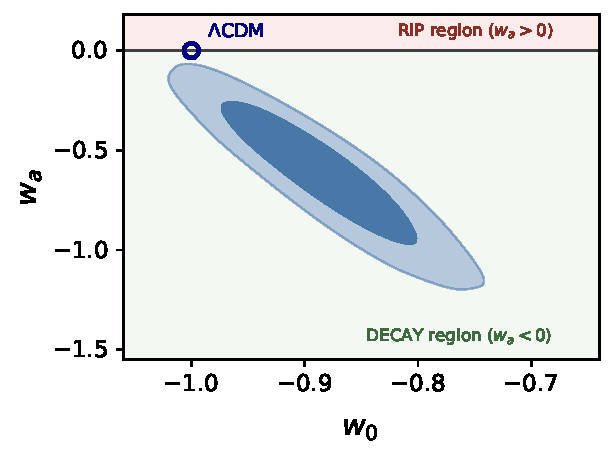
\includegraphics[width=0.85\columnwidth]{../runs/phase2/f2_d0_fate_partition.pdf}
\caption{D0+CPL+P1 posterior over the fate partition. The fate boundary
$\wa=0$ has zero width; \lcdm{} sits exactly on it.}\label{fig:partition}
\end{figure}

Propagating every sample through the classifier yields Table~\ref{tab:d0fate}:
$P(\textsc{decay})=99.82\%\pm0.06\%$, $P(\textsc{rip})=0.18\%\pm0.06\%$
(batch-means errors), zero \textsc{other}, zero boundary flags. Under the
frozen rule that sub-percent tails require a second sampling calculation,
nested sampling gives a consistent weighted point estimate,
$P(\textsc{rip})=\NestedDzeroRipPct\%$. Across three independent seeds, the
between-seed standard deviation is $\NestedDzeroRipSeedSdPct$ percentage
points and the range is $\NestedDzeroRipMinPct$--$\NestedDzeroRipMaxPct\%$.
The previously quoted $0.038\%$ binomial standard error describes only a
fixed-seed equal-weight resample; it is not run-to-run nested-sampling
uncertainty and is therefore not used as an error bar. The weighted nested
\textsc{other} mass is $\NestedDzeroOtherPct\%$, below the registered budget.

\begin{table}[t]
\caption{Fate probabilities, D0+CPL+P1. \emph{Caution: the direction component
of this verdict is uninformative under the null (Sec.~\ref{sec:null}).}}
\label{tab:d0fate}
\begin{tabular}{lcc}
Class & $P$ & thermodynamic class \\
\hline
\textsc{decay} & $99.82\%\pm0.06\%$ & heat-death-compatible \\
\textsc{rip} & $0.18\%\pm0.06\%$ (nested $\NestedDzeroRipPct\%$) & non-heat-death \\
\textsc{ds} & 0 (grammar artifact; Sec.~\ref{sec:fparam}) & heat-death-compatible \\
\textsc{other}/boundary & 0 / 0 & --- \\
\end{tabular}
\end{table}

Two seeds of unease belong here. First, for CPL against \lcdm{}, the
three-seed mean is $\ln B=\NestedLnB$. The between-seed SD is
$\NestedLnBSeedSd$, with range $[\NestedLnBMin,\NestedLnBMax]$. The three
per-run internal dynesty errors span $\NestedLnBInternalMin$--
$\NestedLnBInternalMax$. Bayesian evidence \emph{favors}
\lcdm{} while $\Delta\chi^2$ disfavors it at $2.25\sigma$---a live Lindley
phenomenon~\cite{Lindley1957}, developed as a fragility axis in Sec.~\ref{sec:fstat}. Second,
$P(\textsc{ds})=0$ exactly: strict de Sitter asymptotics is a measure-zero
locus of CPL parameter space, so this zero was decided by the parametrization
before any photon arrived. Before interpreting Table~\ref{tab:d0fate} at all,
however, one must ask what such a table looks like when the truth is exactly
\lcdm{}---the subject of the next section.

\section{Repeated-data calibration}\label{sec:null}
\subsection{Boundary-truth calibration}

We are unaware of a published repeated-\lcdm{}-mock calibration of a posterior
cosmic-fate class probability using the same end-to-end inference pipeline. We
first generated 100 mock datasets whose truth is the \lcdm{} best fit to D0.
A separately frozen extension appended 400 without optional stopping, giving
\NullFiveN{} noisy realizations in total. Noise is drawn from the exact
likelihood covariances (SN $1657\times1657$; BAO $13\times13$; CMB prior
$3\times3$), and every mock is processed by the same CPL+P1 pipeline. A
separate zero-residual realization, excluded from the finite null
distribution, makes all three $\chi^2$ values vanish at the truth and closes
the mock--likelihood loop.

Because the \lcdm{} truth sits on the zero-width CPL fate boundary, local
regular asymptotics predict the heat-death-compatible posterior mass to
approach $U(0,1)$ across repeated realizations: the local likelihood must be
calibrated, the boundary locally linear, and the prior absolutely continuous
with no point mass on \lcdm{}. Under those conditions a direction verdict is correct in
$\sim50\%$ of mocks. This is a property of the specified decision problem,
not a statement that pipeline quality is irrelevant and not a universal
limit on Bayesian procedures. Spike-and-slab priors, explicit \lcdm{} model
probability, curved boundaries, or misspecified posterior widths change the
result (Appendix~\ref{app:boundarystats}).
These predictions were logged mid-campaign (at ${\sim}17$ of 100 mocks),
before the original campaign completed and before the zero-residual run.
They all passed at the historical 100-mock checkpoint. The public extension
did not assume that its original $0/100$ lower-tail count would remain zero.
In the pooled campaign, \NullFiveDirectionK/\NullFiveN{}
($\NullFiveDirectionPct\%$, exact 95\% interval
$[\NullFiveDirectionLowPct,\NullFiveDirectionHighPct]\%$) have
$P(\mathrm{heat})>0.5$, and the complete $P(\mathrm{heat})$ distribution
remains compatible with $U(0,1)$ (KS $p=\NullFiveKSp$;
Fig.~\ref{fig:null}). The maximum \textsc{other} and boundary fractions are
\NullFiveOtherMaxPct\% and \NullFiveBoundaryMaxPct\%, respectively.
The zero-residual mock returns $52/48$. Its data vector equals the truth, but
its likelihood covariance remains finite; it is a closed-loop diagnostic,
not a zero-uncertainty experiment. The result isolates the role of boundary
geometry within this continuous CPL analysis.

The null distribution also supplies the calibrated reading of the real data.
The minimum null Big Rip probability is now
\NullFiveRipMinPct\%, slightly below the observed \DzeroRipPct\%;
\NullFiveK/\NullFiveN{} mocks satisfy
$P(\textsc{rip})_{\rm mock}\le P(\textsc{rip})_{\rm obs}$.
Thus the historical v1.x statement ``below every realization'' was correct
for its first 100 mocks but does not survive the higher-resolution extension.
The registered conditional plus-one value is
$\hat p=(\NullFiveK+1)/(\NullFiveN+1)=\NullFivePlusOne$, with the exact
two-sided 95\% Clopper--Pearson interval
$[\NullFiveCPLow,\NullFiveCPHigh]$ for the underlying fitted-truth tail
probability.
The asymptotic Wilks route gives $p=0.024$, but the statistics are not
equivalent: the mock campaign ranks the one-sided posterior mass
$P(\wa>0\mid D)$ within a CPL pipeline, whereas Wilks tests the point
$(-1,0)$ against a two-parameter CPL alternative. Their numerical agreement
is a useful qualitative cross-check, not two independent measurements of the
same tail. The correct summary of Table~\ref{tab:d0fate} is therefore
two-layered: \emph{the CPL direction probability has the registered uniform
null distribution, while the real data lie unusually deep in its anti-rip
tail and also disfavor point-\lcdm{} by a distinct likelihood-ratio test.}
What that signal does and does not imply about the actual fate is the
subject of the fragility matrix.

\begin{figure}[t]
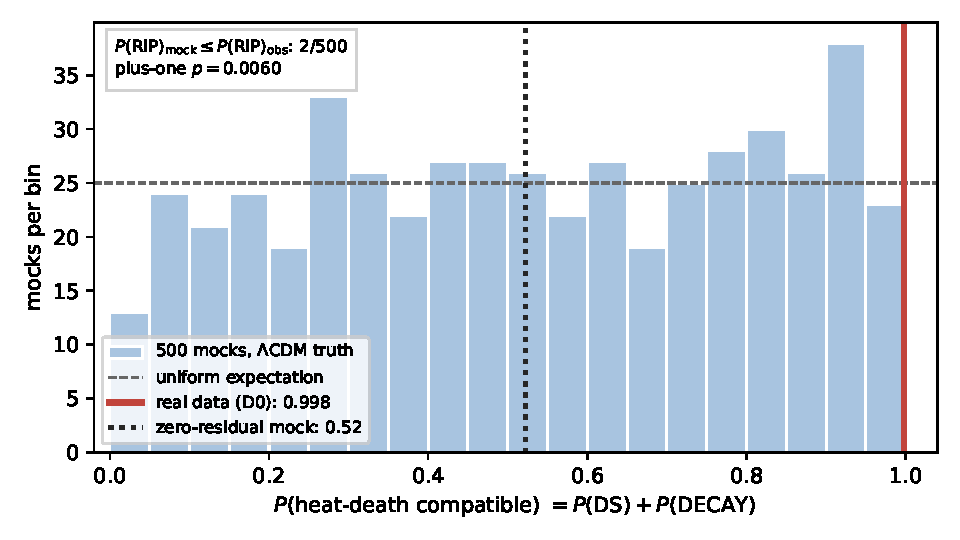
\includegraphics[width=0.95\columnwidth]{../runs/prd_extension/null500/null500_histogram.pdf}
\caption{The completed 500-mock null calibration. Under \lcdm{} truth the
heat-death-compatible posterior mass is consistent with $U(0,1)$
(KS $p=\NullFiveKSp$) for continuous CPL+P1; the excluded zero-residual
diagnostic returns 52/48. Two mocks have
$P(\textsc{rip})\le P(\textsc{rip})_{\rm obs}$; the red line marks the
observed heat-death-compatible mass.}\label{fig:null}
\end{figure}

\subsection{Off-boundary power}\label{sec:power}

Null calibration at the $\wa=0$ boundary does not show how quickly the
statistic becomes informative away from that boundary. The extension
therefore froze six CPL truths at
$\wa=\{-0.60,-0.30,-0.15,+0.15,+0.30,+0.60\}$. At each value all other
parameters were reprofiled against D0 before any of its 100 noisy mocks were
generated. Direction power is the fraction placing more than one half of the
posterior on the truth-consistent thermodynamic side. One-sided depth power
is the fraction rejected at $\alpha=0.05$ against the completed 500-mock null
CDF. Table~\ref{tab:power} reports exact binomial intervals.

\begin{table*}[t]
\caption{Registered truth-specific power. $\Delta\chi^2$ is relative to
the best of the six constrained D0 truth fits, not a common distance from the
fate boundary. Brackets are exact 95\% binomial intervals. The ``false''
column is the fraction placing majority mass on the opposite side.}
\label{tab:power}
\scriptsize
\begin{tabular}{lrrlccc}
Truth & $\wa$ & $\Delta\chi^2$ & correct side &
direction power & depth power & false-sign fraction \\
\hline
wam060 & $-0.60$ & \WpWamSixtyDeltaChi & heat &
\WpWamSixtyDirection & \WpWamSixtyDepth & \WpWamSixtyFalse \\
wam030 & $-0.30$ & \WpWamThirtyDeltaChi & heat &
\WpWamThirtyDirection & \WpWamThirtyDepth & \WpWamThirtyFalse \\
wam015 & $-0.15$ & \WpWamFifteenDeltaChi & heat &
\WpWamFifteenDirection & \WpWamFifteenDepth & \WpWamFifteenFalse \\
wap015 & $+0.15$ & \WpWapFifteenDeltaChi & \textsc{rip} &
\WpWapFifteenDirection & \WpWapFifteenDepth & \WpWapFifteenFalse \\
wap030 & $+0.30$ & \WpWapThirtyDeltaChi & \textsc{rip} &
\WpWapThirtyDirection & \WpWapThirtyDepth & \WpWapThirtyFalse \\
wap060 & $+0.60$ & \WpWapSixtyDeltaChi & \textsc{rip} &
\WpWapSixtyDirection & \WpWapSixtyDepth & \WpWapSixtyFalse \\
\end{tabular}
\end{table*}

Both registered outer-point alternatives pass the predeclared 0.80 direction
gate, so the justified positive claim is that the direction classifier is
powerful under those two alternatives. This is not a global statement:
direction power at $\wa=+0.15$ is $0.77$, and inner-point depth power is only
$0.18$--$0.33$. Moreover, the six generating truths have observed-D0
profile penalties from $0$ to $39.37$. Figure~\ref{fig:power} therefore shows
truth-specific operating characteristics, not a symmetric effect-size curve.
The registered monotonicity rule merely checks for a reversal with disjoint
exact intervals; no such reversal appears, but that coarse clear result is
not separate evidence of power.

\begin{figure*}[t]
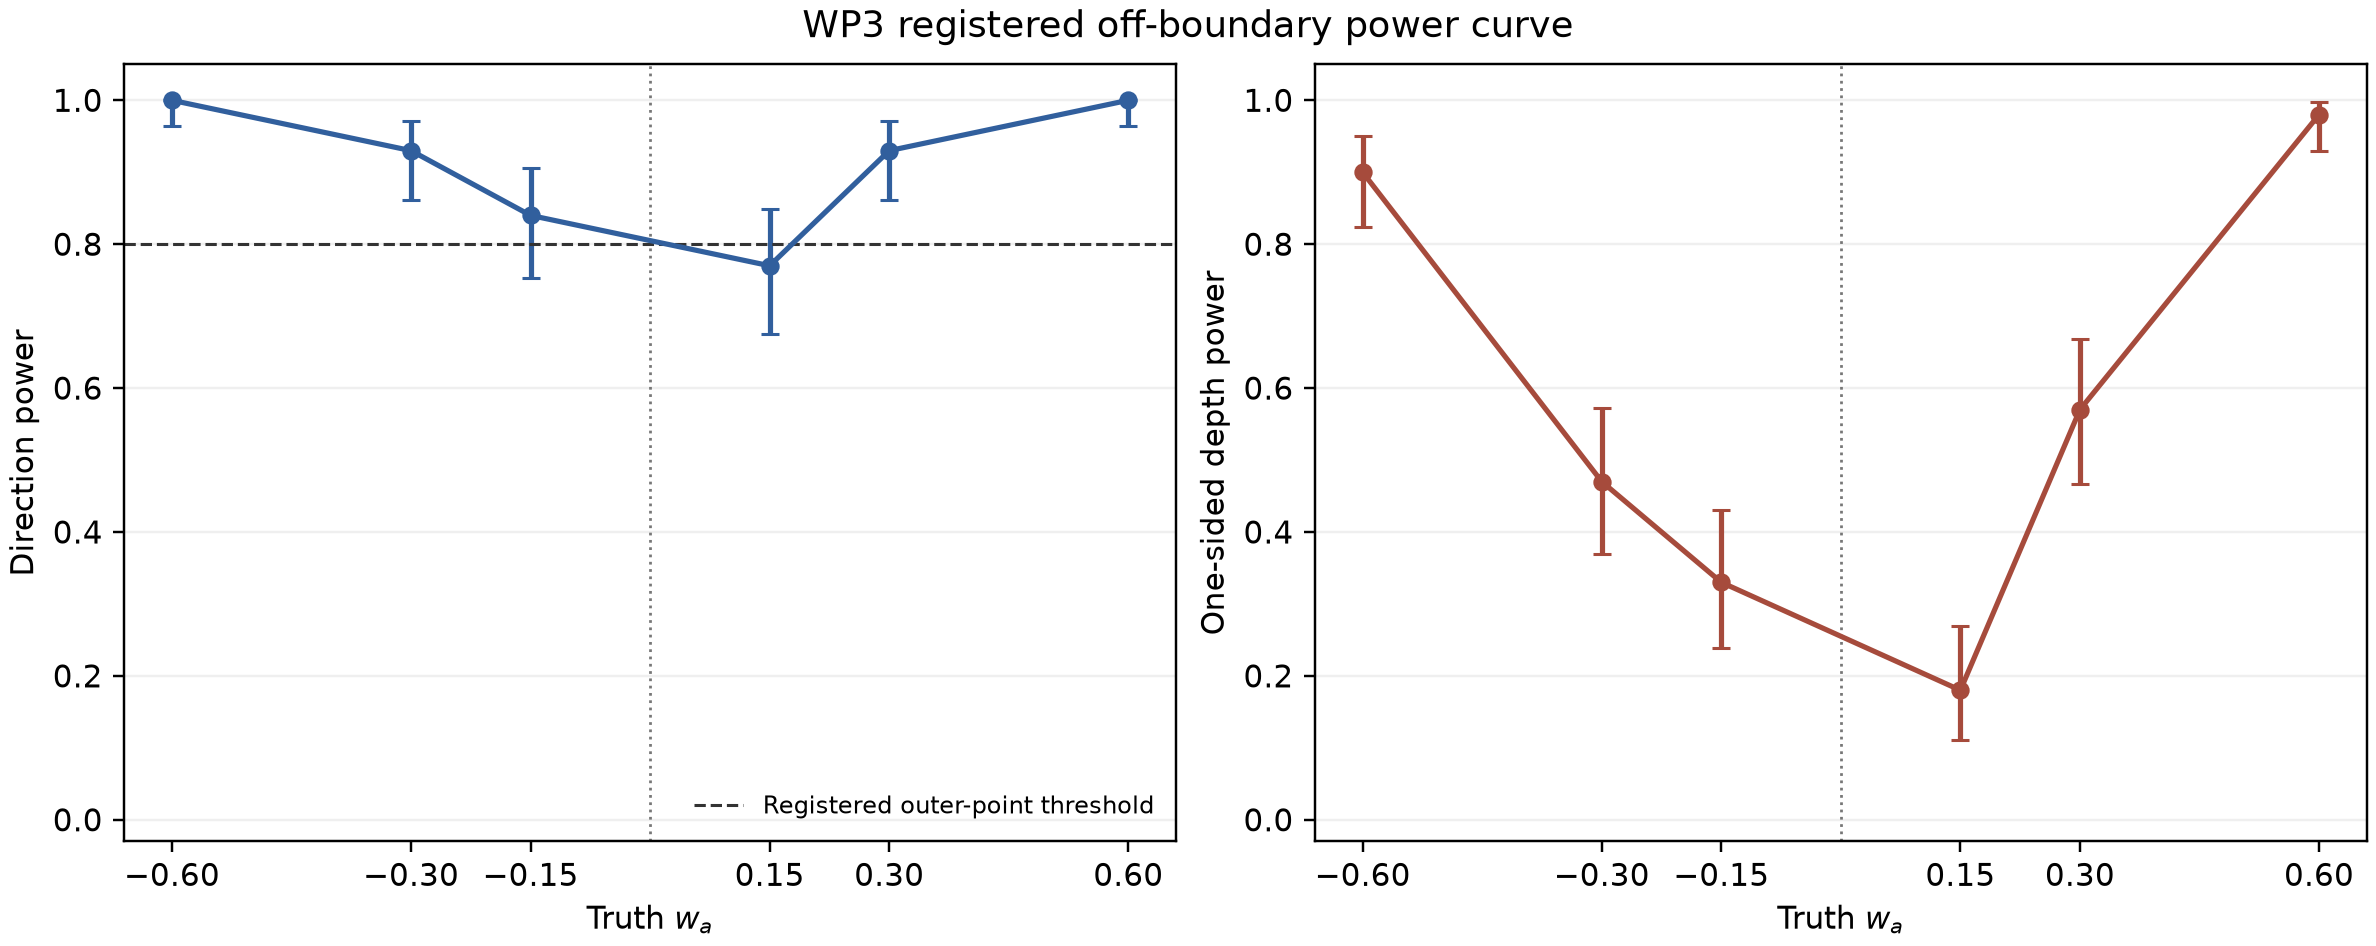
\includegraphics[width=\textwidth]{../runs/prd_extension/wp3_power/power_curve.png}
\caption{Direction and one-sided depth power at six registered constrained
truths. Error bars are exact 95\% binomial intervals; annotations give each
truth's D0 profile $\Delta\chi^2$ relative to the best registered truth.
The unequal profile penalties prevent reading the two sides as equally
supported, symmetric effect sizes.}\label{fig:power}
\end{figure*}

\section{Sensitivity to analysis assumptions}\label{sec:matrix}
\subsection{Data axis}\label{sec:fdata}

Table~\ref{tab:loo} and Fig.~\ref{fig:loo} show the leave-one-out response. The thawing direction
($\wz>-1$, $\wa<0$) survives every ablation---including removal of the CMB
(D2; the CMB prior is replaced by a BBN baryon-density
prior~\cite{Schoeneberg2024}), which \emph{deepens} rather than erases the preference, a point against
the hypothesis that the evidence is purely CMB--low-$z$ tension. The
magnitude, by contrast, is fragile: $\wa$ swings threefold ($-0.55$ to
$-1.72$), and the full combination is more moderate than any
probe-removal subset (D2--D4)---the widely quoted $\wa\approx-0.6$ reflects
partially offsetting dataset pulls. Swapping the supernova compilation
(same model, same priors, same BAO and CMB) moves the \lcdm{} exclusion from
$2.25\sigma$ (Pantheon+) through $2.81\sigma$ (DES-Dovekie) to $3.27\sigma$
(Union3~\cite{Union3}), reproducing the literature's significance
ladder~\cite{Efstathiou2024,HuangCaiWang2025} inside a single
pipeline; the SH0ES anchor alone moves $H_0$ by $+1.37$~km\,s$^{-1}$\,Mpc$^{-1}$ and $\wz$ by $-0.036$
---Hubble-tension leakage into the dark-energy sector. Throughout,
$P(\textsc{rip})$ stays within $\FDataNestedRipMinPct$--$\FDataNestedRipMaxPct\%$:
the direction-level conclusion remains sub-percent for every combination,
but the numerical tail spans $\FDataRip$ dex and is therefore not robust in a
multiplicative sense. Grammar dependence is larger still
(Sec.~\ref{sec:fparam}).

\begin{figure}[t]
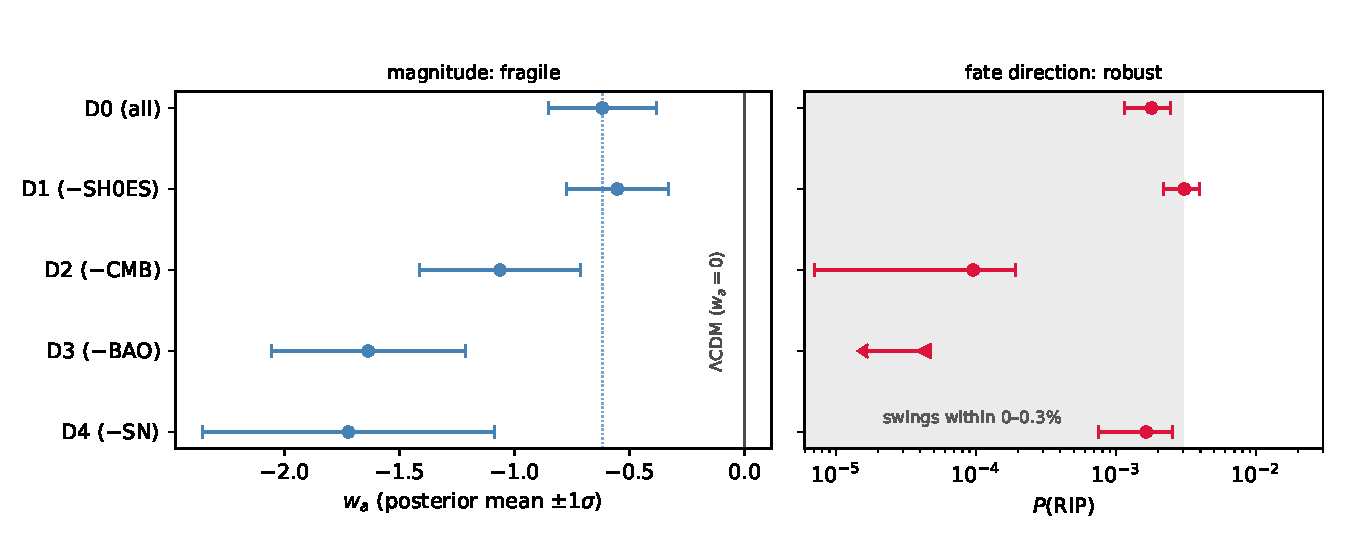
\includegraphics[width=\columnwidth]{../runs/phase3/fdata/f4_loo_forest.pdf}
\caption{Leave-one-out forest (CPL+P1 fixed). Left: the $\wa$ magnitude
swings threefold across dataset ablations, and the full combination (dotted
line) is more moderate than any probe-removal subset (D2--D4). Right: $P(\textsc{rip})$ stays
within $\FDataNestedRipMinPct$--$\FDataNestedRipMaxPct\%$ throughout (shaded); the D3 entry is the
small weighted tail retained by the original nested weights even though its
fixed-seed equal-weight diagnostic contains zero \textsc{rip} draws.}\label{fig:loo}
\end{figure}

\begin{table}[t]
\caption{Leave-one-out (CPL+P1 fixed). Per the frozen sub-percent rule,
the sub-percent entries were recomputed with nested sampling. The weighted
point estimates are consistent in direction with the MCMC values; for D3 the
original weights resolve a small positive tail that the equal-weight diagnostic
rounds to zero. Binomial errors stored with the equal-weight resamples are
numerical resampling diagnostics, not repeated nested-run uncertainties
(per-combination records in the repository).}\label{tab:loo}
\begin{tabular}{lcccc}
Combo & removed & $\wz$ & $\wa$ & $P(\textsc{rip})$ \\
\hline
D0 & --- & $-0.884\pm0.057$ & $-0.62$ & $0.18\%$ \\
D1 & SH0ES & $-0.848\pm0.055$ & $-0.55$ & $\DOneNestedRipPct\%$ \\
D2 & CMB & $-0.853\pm0.067$ & $-1.06$ & $\DTwoNestedRipPct\%$ \\
D3 & BAO & $-0.711\pm0.083$ & $-1.64$ & $\DThreeNestedRipPct\%$ \\
D4 & SN & $-0.43\pm0.22$ & $-1.72$ & $\DFourNestedRipPct\%$ \\
\end{tabular}
\end{table}

\subsection{Prior axis}\label{sec:fprior}

Under the physical priors the question dissolves before data arrive: P2
(pointwise $w(a)\ge-1$, quintessence) and P3 (P2 + thawing) force
$P(\textsc{rip})=0$ \emph{identically}---reported, per the frozen plan, as
``excluded by prior.'' The posterior is pinned into a sliver against the
$w=-1$ wall ($\wz=-0.975$, $\wa=-0.015$), and the wall costs the fit
$\Delta\chi^2=+8.9$ relative to P1: a clean measure of the current tension
between the data and the quintessence hypothesis. P3 adds nothing to P2 on
these data---its extra thawing assumptions are redundant once the pointwise
bound binds. The prior axis reading is therefore maximal:
$\log_{10}P(\textsc{rip})$ spans from $-2.7$ to $-\infty$.

\subsection{Inference-statistic axis}\label{sec:fstat}

The same data, model, and priors yield the fit improvement
$\Delta\chi^2\equiv\chi^2_{\lcdm{}}-\chi^2_{\mathrm{CPL}}=7.44$ (Wilks
$p=0.024$, disfavoring \lcdm) and a three-seed
$\ln B=\NestedLnB$ (between-seed SD $\NestedLnBSeedSd$; Jeffreys-scale
support \emph{for} \lcdm). Nothing is inconsistent: the two statistics ask
different questions, and the Occam penalty of the $15.5$-unit $(\wz,\wa)$
prior area dominates the fit improvement. But the practical consequence is
stark---\emph{whether ``the evidence favors dynamical dark energy'' is
true depends on which inference statistic one grants authority}, and the Bayes
factor's first-order dependence on prior volume makes it a fragility axis of
its own, rarely reported as such. The registered information criteria split
along the same fault line: $\Delta\mathrm{AIC}=-\Delta\chi^2+2\Delta k=-3.4$
sides with the fit, while
$\Delta\mathrm{BIC}=-\Delta\chi^2+\Delta k\ln N=+7.4$ sides with the
evidence ($\Delta k=2$, $N=1673$ data points; negative values favor
CPL)---the direction flip is reproduced within the information-criterion
family itself.

An explicitly model-averaged reading makes the conditioning visible. As an
\emph{exploratory, post-hoc} diagnostic, assign equal prior odds to the
two-model set $\{\lcdm{},\mathrm{CPL}\}$. The measured Bayes factor then gives
$P(\lcdm{}\mid D)=\ModelAvgLCDMPct\%$ and
$P(\mathrm{CPL}\mid D)=\ModelAvgCPLPct\%$; because exact
\lcdm{} is heat-death-compatible, the corresponding model-averaged
compatibility is $\ModelAvgHeatPct\%$. These values are not privileged---they change
with the model set and model prior odds---but they demonstrate why the
continuous-CPL 50/50 boundary result cannot be promoted to a universal
Bayesian claim.

\subsection{Parametrization axis}\label{sec:fparam}

The four converged parametrizations are sensitivity probes, not contestants
in a common-prior model comparison. Their archived chain-minimum AIC values
are descriptively similar (Appendix~\ref{app:fitgrammar}), but those minima
are neither dedicated optimizations nor model evidences. Related in-window
degeneracies are known for overlapping two-parameter families
\cite{Wolf2025}; they do not establish equal model probability for this set.

The four fits do \emph{not} have identical priors. Their coordinate
dimensions, early-matter-domination constraints, and induced measures on
functions and fates differ. A deterministic P1 prior audit makes the baseline
explicit: prior $P(\textsc{rip})$ is $25.8\%$ (CPL), $40.0\%$ (JBP),
$\BAPriorRipPct\%$ (BA), and $\BINPriorRipPct\%$ (BIN4). The likelihood strongly suppresses the
rip in CPL, JBP, and BA, whereas BIN4 remains close to its native prior fate
balance. The residual posterior is therefore strongly grammar-dependent.
The divergent-future CPL and JBP families deliver
near-certain \textsc{decay}; bounded-future BA retains a small
\textsc{rip} component; and frozen-future BIN4 returns
$\BINRipPct\%$ \textsc{rip} and $\BINDecayPct\%$ \textsc{decay}, with strict
\textsc{ds} mass zero.
Its fate-controlling bin is measured as $w_1=-1.000\pm0.044$. Under A-005,
$\BINBoundaryPct\%$ of BIN4 posterior mass is reported as boundary-adjacent
without changing its exact fate label. The binned reconstruction also relocates the
finite-redshift signal: the low-$z$ bin is \lcdm-consistent and the deviation
lies at $z\in[0.7,1.5]$ ($w_3=-1.53\pm0.20$). Thus CPL's
$\wz\approx-0.88$ is partly the transport of a mid-$z$ signal to $z=0$ by a
linear grammar.

A post-hoc matched-prior audit stops before importance weighting. On the
declared seven-point $w(a)$ grid, the CPL, JBP, and BA pushforwards occupy
different two-dimensional supports and BIN4 occupies a three-dimensional
support: the grid reaches only $z=1$, so its summary is
$(w_3,w_2,w_1,w_1,w_1,w_1,w_1)$ and contains no $w_4$ coordinate. Their
common intersection contains only constant histories and has
probability zero under every continuous native prior. A nondegenerate common
target is therefore not dominated by all four pushforwards; diagonal
covariance regularization would manufacture overlap rather than identify a
matched measure. A-004 accordingly terminates the reweighting audit and
withholds all matched fate probabilities.

Among the four fitted parametrizations,
$P(\textsc{rip})$ spans $\GrammarRipMinPct$--$\GrammarRipMaxPct\%$ and
heat-death compatibility spans
$\GrammarHeatMinPct$--$\GrammarHeatMaxPct\%$. These ranges describe the
response of the complete native-prior analyses; they are not a posterior over
parametrizations or a universal model-uncertainty interval.

\begin{table*}[t]
\caption{Grammar-specific induced prior fate mass and posterior fate
probabilities (D0 fixed; A-005 corrected semantics). The CPL posterior row uses the
generic cross-grammar background machinery and agrees with the baseline
within Monte Carlo error. The rows use different native coordinate priors and
are a sensitivity audit, not a common-prior model comparison.}\label{tab:grammar}
\scriptsize
\begin{tabular}{lccccc}
Grammar & prior $P(\textsc{rip})$ & posterior $P(\textsc{rip})$ &
posterior $P(\textsc{decay})$ & posterior $P(\textsc{ds})$ &
posterior $P(\text{heat-death})$ \\
\hline
CPL & $25.8\%$ & $0.21\%$ & $99.79\%$ & $0$ & $99.8\%$ \\
JBP & $40.0\%$ & $0.79\%$ & $99.21\%$ & $0$ & $99.2\%$ \\
BA & $\BAPriorRipPct\%$ & $\BARipPct\%$ & $\BADecayPct\%$ & $0$ & $\BADecayPct\%$ \\
BIN4 & $\BINPriorRipPct\%$ & $\BINRipPct\%$ & $\BINDecayPct\%$ & $0$ & $\BINDecayPct\%$ \\
\end{tabular}
\end{table*}

\section{Partial identification of the future}\label{sec:partialid}
\subsection{Transported information and the direct-support boundary}\label{sec:ah}

Where do the data stop speaking? In the binned grammar the posterior-to-prior
information $D_{\rm KL}[p(w(a))\|\pi]$ is $\KLbinA$, $\KLbinB$, $\KLbinC$, and $\KLbinD$
nat in the four bins (Fig.~\ref{fig:horizon})---the frozen $0.1$-nat horizon
is never crossed inside the observed window: the compressed CMB lever arm
constrains the highest-redshift bin weakly but above threshold. The registered
metric must then be applied to the registered future rule. BIN4 freezes
$w(a>1)=w_1$, so both its posterior and prior are inherited from $w_1$ and
the future KL remains $\KLbinA$ nat. Thus $a_h$ is \emph{not reached};
reporting $a_h=1$ would be inconsistent with the registered metric.

A separate and scientifically important statement does hold: $a=1$ is the
boundary of \emph{direct observational support}. The nonzero KL plotted for
$a>1$ was learned about $w_1$ at $a\le1$ and transported into the future by
the BIN4 freezing rule. CPL transports information differently. Thus future
fate is not supported by direct likelihood evaluations at $a>1$, even though
the posterior-to-prior KL of the extrapolated function need not vanish.

\FloatBarrier
\begin{figure}[!ht]
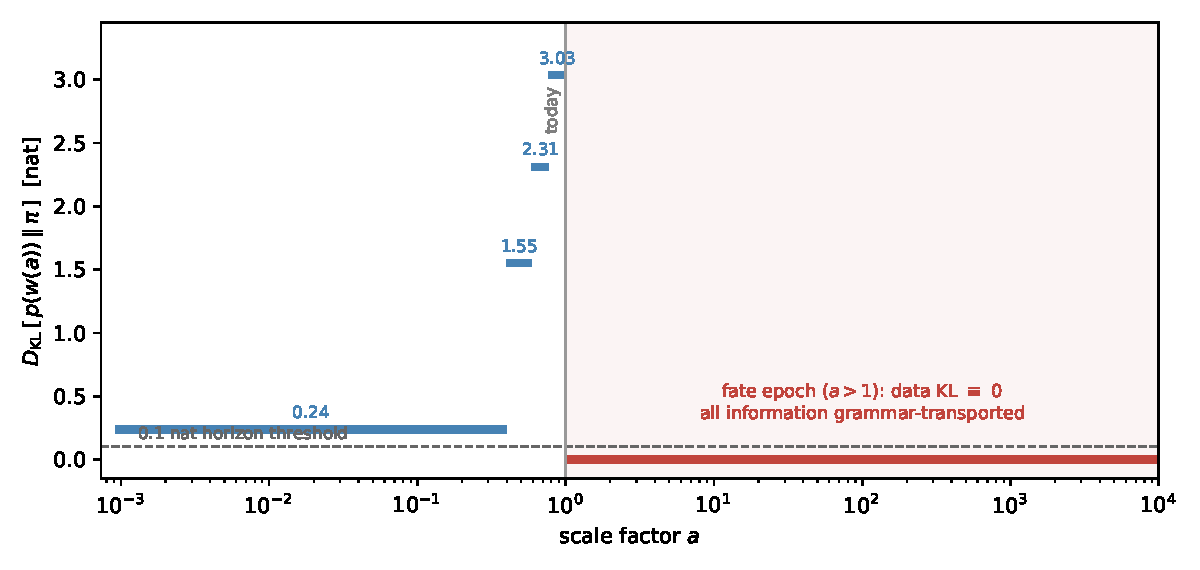
\includegraphics[width=\columnwidth]{../runs/phase3/fparam/f6_constraint_horizon.pdf}
\caption{Constraint horizon (BIN4): posterior-to-prior information in
$w(a)$ per bin. The dashed future segment is the $w_1$ KL inherited by the
BIN4 freezing rule, not direct future information. The frozen $0.1$-nat
threshold is never crossed, so the registered result is $a_h$: not reached.
The vertical line at $a=1$ marks the distinct boundary of direct
observational support.}\label{fig:horizon}
\end{figure}
\FloatBarrier

\subsection{Direct future-continuation audit}\label{sec:continuation}

The constraint-horizon calculation diagnoses transported information but does
not by itself hold the observed history fixed while changing only the future.
The prospectively specified function-space extension performs that stronger
test. It fits a common seven-node grammar, with four nodes at $a\le1$
and three at $a=1.5,2,4$, using a properly normalized truncated correlated
prior. All five registered hyperparameter settings converge, and the inference
implementation passes simulation-based calibration on \WPSevenSBCN{} prior-
predictive datasets: all datasets converge, all registered 50\% and 90\%
coverage counts pass, and no rank test is rejected after Holm correction.

For the primary setting, the frozen continuation gives
$P(\textsc{rip})=\WPSevenPrimaryRipPct\%$. Across the five settings this moves
to \WPSevenRipMinPct--\WPSevenRipMaxPct\%. This variation is not evidence that
the data measure the remote future node. After conditioning analytically on the
four observed-history nodes, the 40-bin posterior-to-prior KL of the final-node
residual is only \WPSevenResidualKL{} nat in the primary setting and never
exceeds \WPSevenResidualKLMax{} nat. The nonzero marginal future-node
information is therefore principally a consequence of the global spline and
its prior correlations, not an observation at $a>1$.

The fixed-history continuation audit takes the same \WPEightRows{} source rows (native weight
\WPEightNativeWeight) and changes only the continuation beyond $a=1$.
The history, every current-background observable, and the likelihood remain
identical to machine precision. Table~\ref{tab:continuations} reports the
registered families. C0 reproduces the seven-node continuation; C1 holds the present value constant; C2 relaxes
smoothly to \lcdm{}; and C3 draws a matched free asymptote. The descriptive
envelope is $P(\textsc{rip})=\WPEightEnvelopeRipMinPct\%$--
$\WPEightEnvelopeRipMaxPct\%$. The continuation families have no probability
measure, so this range is neither a credible interval nor a model average.

The sharp partial-identification endpoint is stronger than the envelope:
\WPEightTwoSidedPct\% of the native source-history weight has support set
$\{\textsc{rip},\mathrm{heat}\}$ across the registered continuations. Thus the
observed history alone identifies neither thermodynamic side. This conclusion
is conditional on the registered kinematic continuation set; the paths are not
asserted to arise from stable, covariant microphysical dark-energy theories.

\begin{table}[!ht]
\caption{Future-continuation audit. All rows share exactly the same fitted
$a\le1$ history. C2 is identical for registered transition scales
$\tau=0.5,1,2$; the three C3 settings remain approximately balanced.}
\label{tab:continuations}
\begin{tabular}{lll}
Family & future rule & $P(\textsc{rip})$ \\
\hline
C0 & frozen FS7 & $\WPEightCZeroRipPct\%$ \\
C1 & present constant & $\WPEightCOneRipPct\%$ \\
C2 & relax to $w_\infty=-1$ & $0\%$ \\
C3 & free asymptote & $49.95$--$50.04\%$ \\
\end{tabular}
\end{table}
\FloatBarrier

\section{Synthesis and discussion}\label{sec:summary}\label{sec:discussion}

\begin{table*}[t]
\caption{The eight-axis fragility matrix. Each row varies one audit package or
axis and reports the response of the fate verdict. The grammar row necessarily
couples functional form, native dimension, and its registered coordinate prior.}
\label{tab:matrix}
\scriptsize
\centering
\resizebox{\linewidth}{!}{%
\begin{tabular}{llll}
\toprule
Axis & knob & response & verdict \\
\midrule
SN compilation & Pantheon+/Dovekie/Union3 & \lcdm{} exclusion $2.25\!-\!3.27\sigma$ & magnitude fragile \\
SH0ES anchor & in/out & $H_0$ ${+}1.37$~km\,s$^{-1}$\,Mpc$^{-1}$; $\wz\,{-}0.036$ & leakage; direction stable within CPL \\
CMB information & CPL compressed/full benchmark & stable $-0.5\sigma$ discount & BIN4 remains compressed-only \\
Dataset ablation & D1--D4 & $\wa\in[-1.72,-0.55]$; $P(\textsc{rip})\,\FDataNestedRipMinPct\!-\!\FDataNestedRipMaxPct\%$ & direction stable; tail $\FDataRip$ dex \\
Prior & P1/P2/P3 & $P(\textsc{rip})$: $0.18\%\to 0$ (excluded) & prior decides \\
Statistic & $\Delta\chi^2$ vs $\ln B$ & $2.25\sigma$ against vs.\ $\ln B=\NestedLnB$ (CPL/\lcdm) & conditioning flips \\
Grammar & four native-prior fits & $P(\textsc{rip})$ $0.21\to49.96\%$ & dominant axis \\
Truth position & \lcdm{} in continuous CPL & verdict $\sim U(0,1)$; zero-residual 52/48 & conditional null law \\
\bottomrule
\end{tabular}
}
\end{table*}

The reported log-span metrics are collected in
Table~\ref{tab:formalfragility}; they are not replaced by the broader
eight-axis narrative matrix. The exact zero imposed by P2/P3 makes the prior
span infinite. No original-weight $F_{\rm data}$ point is zero: D3 retains a
small positive tail even though its equal-weight diagnostic contains zero
\textsc{rip} draws. A finite-run zero is not promoted to a mathematical zero.

\begin{table}[t]
\caption{Reported fragility measures, in dex. The parametrization row covers
the four converged native-prior fits.}
\label{tab:formalfragility}
\begin{tabular}{lcc}
Axis & $P(\textsc{rip})$ span & $P(\mathrm{heat})$ span \\
\hline
$F_{\rm prior}$ & $\FPriorRip$ & $\FPriorHeat$ \\
$F_{\rm param}$, fitted four & $\FParamFitsRip$ & $\FParamFitsHeat$ \\
$F_{\rm data}$ & $\FDataRip$ & $\FDataHeat$ \\
\end{tabular}
\end{table}

Table~\ref{tab:matrix} assembles the audit. For D0 within CPL+P1, the
posterior-tail mock rank and the non-equivalent Wilks statistic both lie near
the percent level: the 500-mock plus-one value is \NullFivePlusOne, while
Wilks gives $0.024$. Across D1--D4, the anti-rip posterior direction remains
sub-percent within the same CPL pipeline, but those variants were not
separately null-calibrated and the tail magnitude spans $\FDataRip$ dex.
Quantities specifically about fate---which endpoint, with what
probability---also respond strongly to theory-side choices that the current
likelihood does not directly constrain.

\emph{Three layers.} The audit resolves the fate question into three layers
with different epistemic status. (i) \emph{Direction}: within the continuous
CPL decision problem, the fate-side posterior mass approaches a uniform null
distribution when the truth lies on the local \lcdm{} boundary. This statement
does not transfer automatically to BIN4 or to explicit model averaging.
(ii) \emph{Depth}: within CPL+P1 and the adopted compressed-CMB likelihood,
the D0 posterior lies in the anti-rip tail of the fitted-truth mock distribution
(\NullFiveK/\NullFiveN{} null mocks at least as deep,
$\hat p=\NullFivePlusOne$, exact 95\% interval
$[\NullFiveCPLow,\NullFiveCPHigh]$); the non-equivalent Wilks test gives
$p=0.024$. The off-boundary experiment additionally shows strong direction
power at the two registered outer truths, but materially weaker inner-point
direction and depth power. This is a pipeline-conditional finite-redshift
preference, not a calibration of data systematics, likelihood compression, or
cross-model uncertainty. Across D1--D4 the anti-rip posterior direction remains
sub-percent within CPL+P1, but these variants were not separately
null-calibrated. Separately, BIN4 places its largest in-window departure at
$z\in[0.7,1.5]$. (iii) \emph{Translation}: converting finite-redshift
information into a fate probability additionally requires an extrapolation
rule and induced prior measure that observations do not directly constrain.
The exact continuation audit makes this last layer constructive: without
altering any current-background observable or likelihood value, every weighted source history admits both
rip and heat-death-compatible registered continuations.

\emph{Why the fragility is structural, not accidental.} The fate map is a
\emph{discontinuous} functional of parameters that observation constrains
only \emph{continuously}: \textsc{rip} and \textsc{decay} are separated by a
zero-width boundary, and \lcdm{} sits on it. Under regular continuous-model
asymptotics, repeated-data class probabilities remain uniform when the truth
is exactly on a locally linear boundary, even as the likelihood narrows. This
statement is conditional: a discrete \lcdm{} component, model averaging,
nonregular priors, or a physically derived theory changes the inferential
object. In that qualified sense the result is a quantitative instance of the
underdetermination of dark energy articulated in
Refs.~\cite{WolfFerreira2023,WolfRead2026}, not a no-go theorem for every
future Bayesian procedure.

\emph{What would change the situation.} More precise distance data can narrow
the finite-redshift function and may reveal that the truth is off the
boundary, but observations made today cannot directly sample $a>1$. The
registered KL horizon is not reached; the relevant limitation is instead the
direct-support boundary at $a=1$. Extrapolation is licensed by trusted theory,
not by fit quality alone. CPL and its cousins are
more than raw curve fitting---they are compressions calibrated against
quintessence-class dynamics inside the
window~\cite{CaldwellLinder2005,Linder2006,dePutterLinder2008}---but a
calibrated compression is still not a theory: the calibration certifies
fidelity to a model class over the fitted range, and extending that fidelity
to $a>1$ is precisely the adoption of the class as a prior---an axis this
audit prices (Sec.~\ref{sec:fprior}). A physically derived dark-energy model
(a specific potential, a symmetry argument) would convert fate back into a
derivation---then data would test the theory inside the window and the
theory would carry the license beyond it. Until then, fate probabilities
remain conditional predictions of the adopted model class.

The continuation result should be read at the same level. C0--C3 are smooth
background expansion rules, not demonstrations that every path arises from a
stable covariant field theory with acceptable perturbations. A specified
microphysical theory may link the present state to a unique future through its
equations of motion and thereby exclude most or all of these continuations.
Our result therefore establishes partial identification when no such dynamical
license is supplied; it does not prove that cosmic fate is unknowable in every
physical theory.

\emph{Relation to the recent fate literature.} Papers reporting
$P(\text{fate})$ have always been conditional on a parametrization or physical
model. Earlier work explicitly replaced CPL with a bounded future
parametrization, and recent studies examine multiple parametrizations or
specific scalar-field scenarios
\cite{LiFate2012,AndreiIjjasSteinhardt2022,Gialamas2025,Wolf2025}. These are
scientifically meaningful conditional calculations. Our narrower contribution
is to report the induced prior fate mass, cross-grammar sensitivity, and
fitted-truth null calibration in one audit. Table~\ref{tab:matrix} is therefore
a finite, non-exhaustive sensitivity budget, not a universal model-uncertainty
interval. The framework---local preregistration, null calibration, and declared
assumption axes---can be adapted to other inferences whose conclusions lie
beyond their data window.

\emph{Limitations.} All significances inherit the compressed-CMB condition
(priced at $\approx0.5\sigma$; A-001). That condition is mildest for
CPL-like histories, for which the distance priors were
validated~\cite{ChenHuangWang2018}; for the binned grammar, whose
high-$z$ bin can depart further from $\Lambda$, extraction-side validity
is an additional inherited assumption. The analysis is background-only: it
does not evolve CMB spectra, dark-energy perturbations, or late-time growth.
Growth information could shift the finite-redshift posterior, but it would not
directly observe $a>1$. For BIN4, we impose the hard gate
$\rho_{\rm DE}/\rho_m(z=1059)<0.01$; the archived posterior has zero weighted
violating mass and a maximum sampled ratio $8.62\times10^{-5}$; this check does
not turn the distance prior into a full-CMB likelihood.

The four converged parametrizations are neither exhaustive nor a model
average. Their native priors induce different measures on functions and fates,
and their pushforwards have incompatible supports on the declared common
summary. Consequently, their probability span is a sensitivity diagnostic,
not a credible interval or universal model-uncertainty bound. The repeated-
data calibration is likewise conditional on fitted-truth \lcdm{} analyzed
with CPL+P1; it does not calibrate model misspecification or every grammar.
The registered continuations are kinematic, and heat-death compatibility is a
coarse endpoint grouping rather than a calculation of vacuum decay, black-hole
evaporation, or quantum-gravitational thermodynamics. Further
parametrizations and physical reconstructions remain possible
\cite{Wolf2025}. The work was performed by a single author with AI assistance
under the verification protocol described; residual unknown-unknowns are
bounded only by the public audit trail.

\section{Conclusions}\label{sec:conclusions}

Within CPL+P1 and the adopted compressed-CMB likelihood, the data give a
pipeline-conditional finite-redshift result: \NullFiveK{} of \NullFiveN{}
fitted-truth \lcdm{} mocks are at least as deep as the real CPL tail, giving
$\hat p=\NullFivePlusOne$, while the distinct Wilks test gives $p=0.024$.
This calibration is informative about the specified CPL decision problem, not
about every model or data systematic.

Translation from that result to cosmic fate is assumption-dependent. A
quintessence prior excludes the rip before data are considered, and four
converged parametrizations, each with its native prior, move posterior
$P(\textsc{rip})$ from
$\GrammarRipMinPct\%$ to $\GrammarRipMaxPct\%$ against already different
induced prior masses. These values diagnose sensitivity; they are not a
common-prior model comparison.

The direct-support boundary is $a=1$. In the calibrated seven-node analysis,
the final-node conditional-residual information is only
\WPSevenResidualKL{} nat. Holding the entire observed history fixed, the
registered continuations span
$P(\textsc{rip})=\WPEightEnvelopeRipMinPct\%$--
$\WPEightEnvelopeRipMaxPct\%$, and \WPEightTwoSidedPct\% of source-history
weight admits both fate sides. No probability is assigned to the continuation
families. Thus present observations can produce sharp fate probabilities
within a chosen model, but they do not identify a unique infinite future
without a physical continuation law. This is a background-level partial-
identification result within the registered kinematic class, not an
impossibility theorem for all microphysical theories.

\acknowledgments
This work used \texttt{CAMB}~\cite{CAMB}, \texttt{cobaya}~\cite{cobaya},
\texttt{GetDist}~\cite{getdist}, and \texttt{dynesty}~\cite{dynesty}; we thank
their authors, and the DESI collaboration for the public release of the DR2
cosmology chains used in validation. Generative-AI assistance was provided by
Anthropic Claude Fable 5 and OpenAI Codex (GPT-5) for portions of pipeline
implementation, literature triage, manuscript drafting and editing, and
reproducibility and consistency checks. All AI-assisted material was
critically reviewed under the version-controlled verification protocol
described in Sec.~\ref{sec:prereg}; the tools did not generate or alter
original research data, and all analysis choices, amendment sign-offs, and
final claims are the author's responsibility.

\appendix

\section{Analysis plan and reported scope}\label{app:plan}

The locally frozen original under tag \texttt{prereg-v1} remains archived in
the repository and takes precedence over this summary. It was not deposited
in a third-party registry at freeze time. This appendix records only the
components that contribute to the reported scientific results; amendments are
summarized in Appendix~\ref{app:amendments}.

\emph{Research question.} The declared deliverable was a set of fragility
measures, not a fate discovery. Data-dominated and assumption-dominated
outcomes were both designated as publishable before the first target fate
calculation.

\emph{Model and data.} The analysis treats background expansion only,
$H^2(a)/H_0^2=\Omega_r a^{-4}+\Omega_m a^{-3}+\Omega_k a^{-2}
+\Omega_{\rm DE}f_{\rm DE}(a)$, with flat CPL as the baseline and BA, JBP,
and BIN4 as the converged parametrization-sensitivity set
\cite{BarbozaAlcaniz2008,JBP2005}. D0 combines DESI DR2 BAO, the CMB distance
prior, and Pantheon+ with SH0ES; D1--D4 remove one component at a time, and
the supernova-compilation audit replaces Pantheon+ while holding the other
choices fixed. A prospectively specified extension adds the calibrated
seven-node reconstruction and fixed-history continuation audit.

\emph{Priors and fate rules.} P1 is the baseline native-coordinate prior; P2
adds pointwise $w(a)\ge-1$; P3 adds the phenomenological thawing restrictions.
The classifier priority is \textsc{crunch} $>$ \textsc{rip} $>$ \textsc{ds}
$>$ \textsc{decay} $>$ \textsc{other}, with a 1\% \textsc{other} budget and
a doubled/halved-threshold boundary audit. The operational thermodynamic map
groups \textsc{ds} and \textsc{decay} as heat-death-compatible and
\textsc{rip} and \textsc{crunch} as non-heat-death.

\emph{Statistical and reporting rules.} Chains entering results must satisfy
$R-1<0.01$ on the worst parameter. Sub-percent fate tails require independent
nested-sampling verification. The reported sensitivity measures are the
$\log_{10}$ spans across P1--P3, the four converged parametrizations, and
D0--D4. Repeated-data calibration, model evidence, the constraint-horizon
diagnostic, and exact continuation invariance are reported as distinct
inferential objects rather than interchangeable significances.

\emph{Freeze discipline.} The tagged plan is immutable. Changes are recorded
in an append-only ledger with their trigger and timing relative to data contact.
Exploratory extensions that do not satisfy their completion gates are excluded
from scientific results; their audit records remain in the repository.

\section{Amendment log}\label{app:amendments}

The complete signed ledger is archived in the repository. The entries below
summarize only changes that affect the interpretation or reproducibility of
reported results.

\emph{A-001 (2026-07-03; before fate analysis).} Gate~1 was changed from
matching the official full-\textit{Planck} exclusion significance to matching
published compressed-CMB analyses of the same class. The best-fit-point gate
was unchanged. The pipeline agrees with the official contour, but every
reported significance inherits the measured $\approx0.5\sigma$ compression
discount (Secs.~\ref{sec:data} and \ref{sec:matrix}).

\emph{A-002 (2026-07-06; during the mock campaign).} The invalid requirement
that at least 90\% of boundary-truth mocks favor heat-death compatibility was
replaced by reporting the null distribution itself. For regular continuous
CPL at the \lcdm{} boundary, the predicted class probability is approximately
$U(0,1)$; the completed campaign confirms that conditional result
(Sec.~\ref{sec:null}). The \textsc{other} and boundary budgets were unchanged.

\emph{A-003/A-005 (2026-07-06/21; classifier correction).} The registered
\textsc{other} budget exposed a gap for parametrizations with finite
$w_\infty$. An analytic finite-limit branch was added and later corrected to
the physical boundaries: \textsc{rip} iff $w_\infty<-1$, \textsc{ds} iff
$w_\infty=-1$, and \textsc{decay} iff $w_\infty>-1$; $\epsilon=0.01$ is only
a boundary-adjacent flag. BA and BIN4 were reclassified accordingly. CPL,
JBP, D0--D4, P2/P3, the mock calibration, Wilks statistics, and evidence are
unchanged.

\emph{A-004 (2026-07-21; post-hoc support audit).} On the declared seven-node
summary, CPL, JBP, and BA occupy different two-dimensional supports and BIN4
occupies a three-dimensional support. Their common intersection contains only
constant histories and has probability zero under every continuous native
prior. No nondegenerate common reweighting target therefore exists; matched
fate probabilities are withheld (Sec.~\ref{sec:fparam}).

\emph{A-006/A-007 (2026-07-21/22; scope and provenance).} The insufficient
condition $w_4<0$ was replaced by
$\rho_{\rm DE}/\rho_m(z=1059)<0.01$. The archived BIN4 posterior has zero
weighted violating mass and a maximum ratio $8.62\times10^{-5}$. The ledger
also records the grammar-specific translation of the original early-matter-
domination intent. No reported probability changes under these records, and
BIN4 remains background-only and compressed-CMB-conditioned.

Analyses that did not pass their completion gates are absent from the
scientific results; their exclusion records remain in the repository.

\section{Exploratory in-window fit audit}\label{app:fitgrammar}

Table~\ref{tab:fitgrammar} reports the lowest likelihood $\chi^2$ values in
the archived post-burn-in chains. Common parameters cancel in $\Delta$AIC.
The entries are descriptive chain minima, not dedicated optimizations,
evidences, or model probabilities.

\begin{table}[h]
\caption{Exploratory in-window fit audit.}\label{tab:fitgrammar}
\begin{tabular}{lrrrr}
Grammar & $\chi^2_{\rm chain,min}$ & $\Delta\chi^2$ & $\Delta$AIC & $R-1$ \\
\hline
CPL  & 1489.534 & 0.000 & 0.000 & \RCPL \\
JBP  & 1492.075 & 2.541 & 2.541 & \RJBP \\
BA   & 1491.523 & 1.989 & 1.989 & \RBA \\
BIN4 & 1485.386 & $-4.149$ & $-0.149$ & \RBIN \\
\end{tabular}
\end{table}

\section{Classifier numerics and known edges}\label{app:classifier}

The classifier integrates each posterior sample's background from $a=1$ to
$a_{\max}=10^4$ and applies Sec.~\ref{sec:fate}'s criteria with the frozen
thresholds: \textsc{rip} tail-convergence tolerance $10^{-3}$ (relative
change of $t(a)$ from $a_{\max}$ to $2a_{\max}$); \textsc{ds} tolerance
$|w(a_{\max})+1|<0.01$; \textsc{decay} thresholds
$\rho_{\rm DE}(a_{\max})/\rho_{\rm DE}(1)<0.01$ or
$\rho_{\rm DE}/\rho_m(a_{\max})<1$; A-005 finite-limit boundary-adjacent
tolerance $\epsilon=0.01$. Numerics: the age integral $\int da/(aH)$ is evaluated by
adaptive quadrature on 40 logarithmically spaced panels; the \textsc{crunch}
scan uses a 400-point logarithmic grid in $a$; $\ln f_{\rm DE}$ is capped at
700 before exponentiation to avoid overflow (samples beyond the cap are
already deep in the \textsc{rip} regime). The boundary flag re-runs the
classification with all thresholds doubled and halved and marks any sample
whose label flips.

The implementation passes a ten-case unit suite: \lcdm{}
$\to$ \textsc{ds} (unflagged); phantom $\wa>0$ $\to$ \textsc{rip}; the DR2
best fit $\to$ \textsc{decay}; mild thawing $\to$ \textsc{decay}; a closed,
decaying-DE case $\to$ \textsc{crunch}; finite-limit cases just below,
above, and exactly at $w_\infty=-1$ map to \textsc{rip}, \textsc{decay},
and \textsc{ds}, respectively, with the boundary-adjacent flag raised; and two
\emph{documented limitation cases} of the frozen criteria, constant-$w$
curves with $w=-0.98$ (quasi-$\Lambda$: neither \textsc{ds}-tight nor
decayed at $a_{\max}$) and $w=-1.2$ (power-law phantom: a true finite-time
singularity whose tail convergence at $a_{\max}=10^4$ is slower than the
frozen tolerance), both of which are intentionally routed to \textsc{other},
i.e.\ to the manual-audit channel. Constant-$w$ curves are measure-zero in
the CPL posterior; the posterior mass in the band $|\wa|<3\times10^{-4}$ is
$\sim10^{-3}$, safely inside the 1\% \textsc{other} budget. These edges were
documented before the real-data runs and did not require an amendment; the
distinct gap later exposed by bounded-future grammars did (A-003,
Appendix~\ref{app:amendments}).

Across the four reported parametrizations, the cross-grammar machinery takes
$r_{\rm drag}$ from a \lcdm{} computation (drag-epoch physics treated as
dark-energy independent); this is self-consistent a posteriori even for the
binned grammar, whose free high-$z$ bin sits at $w_4=-1.71\pm0.62$. The A-006
weighted audit gives zero posterior mass above
$\rho_{\rm DE}/\rho_m(z=1059)=0.01$ and a maximum sampled ratio
$8.62\times10^{-5}$; this posterior check does not turn the compressed
distance prior into a full-Planck likelihood.

\section{Mock machinery and zero-residual validation}\label{app:mocks}

The null-calibration truth is the \lcdm{} best fit to D0
($\Omega_m=0.2968$, $H_0=68.81$, $M_B=-19.397$), located by repeated
bounded minimization. Each noisy mock draws one noise realization per
likelihood from the exact covariances used in inference---SN
$1657\times1657$ (stat+sys, retaining rows with $z_{\rm HD}>0.01$ or a
Cepheid calibrator), BAO $13\times13$, CMB
prior $3\times3$---added to the truth's predicted data vectors, and is then
processed by the full CPL+P1 pipeline (MCMC and classifier identical to the
real-data runs). The campaign is a point null---mocks are generated at the
single best-fit truth rather than marginalized over the \lcdm{} posterior.
The historical v1.x checkpoint contained noisy indices 1--100. The frozen
extension replayed the same generator stream and appended indices
101--500 in an isolated result tree; it could not stop early and did not
overwrite the v1.x inputs.
For the direction layer this is sufficient: the uniformity prediction is
truth-value-independent for any truth on the fate boundary
(Appendix~\ref{app:boundarystats}), and every \lcdm{} parameter point sits
on it; the depth-layer floor inherits the usual parametric-bootstrap
caveat of being conditioned on the fitted truth.
Mocks are generated deterministically from a single seed,
so the entire campaign regenerates bit-identically from the repository. A
101st, zero-residual realization (\texttt{mock000}) provides a closed-loop
test: at the truth point all three likelihood $\chi^2$ vanish identically,
verifying the mock--likelihood round trip; its fate verdict (52/48) is the
finite-covariance boundary diagnostic of Sec.~\ref{sec:null}.

Six falsifiable predictions were logged during the original campaign (after
${\sim}17$ of its 100 mocks had been inspected), derived from the
probability-integral-transform argument, before the campaign's completion
and before the zero-residual realization ran:
direction accuracy $50\pm10\%$; $P_{\rm heat}$ consistent with $U(0,1)$;
0--3 of 100 mocks below the real data's $P(\textsc{rip})$;
\textsc{other} and boundary budgets at the $10^{-3}$ level;
\texttt{mock000} near 0.5; and the resulting A-002 trigger. All six were
correct at that historical checkpoint. The extension explicitly declined to
predict that $0/100$ would remain zero: its completed result is
\NullFiveK/\NullFiveN. Per-mock records (501 rows), the completion audit,
the six versioned endpoint blocks, and the batch logs are in the repository.

\section{Boundary calibration statistics}\label{app:boundarystats}

This appendix collects, in an idealized regular-model form, the statistical facts
behind the null calibration of Sec.~\ref{sec:null}: the exact uniformity
result, its closed-form verification, the diagnostics that detect a
\emph{mis}calibrated pipeline, the finite-mock reporting rules, and the
relation to the calibration literature.

\emph{One dimension.} Let $\hat{x}\sim\mathcal{N}(\theta_0,\sigma^2)$ with
posterior $\theta\,|\,\hat{x}\sim\mathcal{N}(\hat{x},\sigma^2)$ (the
calibrated case), and let class $A$ be $\theta>0$ with the truth on the
boundary, $\theta_0=0$. Then $P(A\,|\,\hat{x})=\Phi(\hat{x}/\sigma)=\Phi(Z)$
with $Z\sim\mathcal{N}(0,1)$: by the probability integral
transform~\cite{Rosenblatt1952}, the class probability is \emph{exactly}
$U(0,1)$ across realizations. Numerically ($2\times10^5$ replications):
mean $0.5010$, variance $0.08356$ against the uniform value $1/12\approx
0.08333$, direction rate $0.502$, KS $p=0.16$. Because the class
probability is a continuous functional of the data, its null distribution
has no atom at $1/2$: individual realizations can look arbitrarily
confident while the ensemble verdict remains a fair coin.

\emph{Two dimensions, correlated errors.} In a $(u,v)$ analogue of
$(\wz{+}1,\wa)$ with a D0-like degenerate covariance and a linear fate
score $s=\alpha u+v$ ($\alpha=1.2$, class $s>0$), the same argument applies
to any linear boundary through the truth: $5\times10^4$ replications give
mean $0.5013$, variance $0.08326$, direction rate $0.505$, KS $p=0.058$
(at $5\times10^4$ replications the KS test resolves sub-percent
distortions; this is comfortable agreement).
The CPL fate boundary $\wa=0$ is exactly linear, so the result covers the
geometry of Sec.~\ref{sec:null} up to the non-Gaussianity of the real
posterior---which the full-pipeline campaign tests directly.
The derivation assumes a continuous posterior with no atom on the boundary.
It does not apply unchanged to spike-and-slab priors or Bayesian model
averaging that assigns positive probability to exact \lcdm{}.

\FloatBarrier
\begin{figure}[!ht]
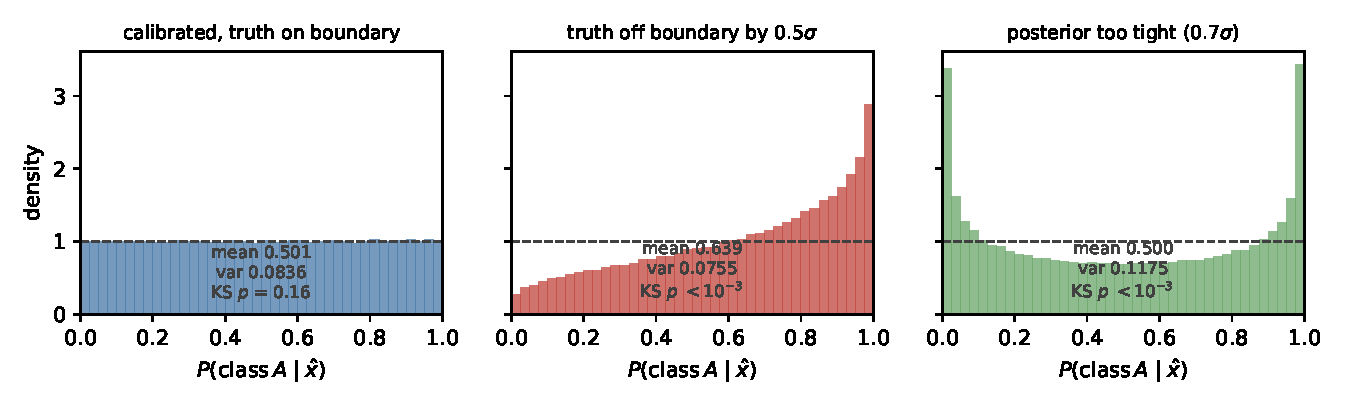
\includegraphics[width=\columnwidth]{figures/figA_boundary_toy.pdf}
\caption{The boundary-calibration toy (Appendix~\ref{app:boundarystats}).
Left: calibrated posterior with the truth on the boundary---class
probabilities exactly uniform. Center: truth off the boundary by
$0.5\sigma$---direction information appears, as it should. Right:
over-confident posterior---mean preserved but variance above $1/12$; the
uniformity diagnostics fail precisely when the pipeline is defective.}
\label{fig:boundarytoy}
\end{figure}
\FloatBarrier

\emph{Diagnostics: when uniformity must fail.} The value of the null test
lies in what breaks it (Fig.~\ref{fig:boundarytoy}). Truth off the
boundary by $0.5\sigma$: mean $0.639$, direction rate $0.692$, KS
$p\approx0$---direction information appears exactly when it exists.
Decision threshold shifted while the truth sits on it: still uniform (KS
$p=0.25$)---only the truth--boundary distance matters. Posterior too wide
(under-confident, $1.5\sigma$): mean stays at $0.500$ but the variance
collapses to $0.0496<1/12$. Posterior too tight (over-confident,
$0.7\sigma$): variance inflates to $0.1175>1/12$. Strongly curved
boundary: KS $p=2.5\times10^{-6}$---uniformity is a locally-linear
statement (the CPL boundary is exactly linear). The triple observed in
Sec.~\ref{sec:null}---accuracy $\approx50\%$, uniform shape, variance
consistent with $1/12$---shows no gross defect of the tested kinds. The
diagnostics respond in distinct directions in the simulations, but a
100-realization campaign retains limited power against mild misspecification.

\emph{Finite-mock reporting rules.} With $k$
of $n$ fitted-truth mocks at or below the real-data statistic, we report the conditional plus-one
estimate $\hat{p}=(k+1)/(n+1)$~\cite{PhipsonSmyth2010} and the exact
two-sided 95\% Clopper--Pearson interval for the underlying tail probability;
a finite-simulation $p$-value is never reported as zero. At the historical
$k=0,n=100$ checkpoint these rules gave $\hat p=0.0099$ and upper bound
$0.0295$. The completed extension has $k=\NullFiveK,n=\NullFiveN$,
$\hat p=\NullFivePlusOne$, and interval
$[\NullFiveCPLow,\NullFiveCPHigh]$. The larger campaign strengthens finite
tail resolution while invalidating the historical ``below every mock''
wording.

\emph{Relation to the calibration literature.} The lineage runs from the
probability integral transform~\cite{Rosenblatt1952} through prequential
calibration~\cite{Dawid1984} and posterior predictive
checking~\cite{Rubin1984,GelmanMengStern1996}. The closest modern relative
is simulation-based calibration~\cite{Talts2018}, which validates posterior
computation via rank uniformity under prior-drawn truths. The present test
differs in both conditioning and target: the truth is \emph{fixed at the
boundary point}, and the calibrated object is a \emph{decision functional
discontinuous there}---the campaign is a null test of the verdict, not of
the posterior machinery (which Gate 1 validates separately). The practical
residue is a reporting discipline matching the three layers of
Sec.~\ref{sec:discussion}: a fate-style claim should state (i) its
direction-layer verdict together with the null distribution of that
verdict, (ii) its depth-layer tail probability under the finite-simulation
rules above, and (iii) the translation-layer conditions---parametrization,
prior, statistic---under which the verdict holds; Table~\ref{tab:matrix}
is the translation layer's error budget.

\section{Data, code, and reproducibility}\label{app:repro}

The repository, \url{https://github.com/shlinawaf717-collab/cosmo_fate}
(archived at Zenodo, \url{https://doi.org/10.5281/zenodo.21332433}),
contains the frozen plan and amendment log, the full pipeline (likelihood configurations,
fate classifier and its unit suite, mock generator, batch drivers, nested
verification), archived thin chains and per-mock records sufficient for the
reported summaries, the figure scripts, and
deterministic audits for induced prior fate mass, in-window chain minima,
model averaging, the registered constraint-horizon metric, the matched-prior
support audit, and the grammar-prior implementation trace. The extension
additionally versions the 500-mock completion and endpoints; the six
truth-specific power fits, completion audit, exact power table, and
profile-$\chi^2$-annotated figure; the seven-node SBC and five-setting
endpoints; and the exact fixed-history continuation audit. All
input data are public: DESI DR2 BAO compressed measurements and covariance;
Pantheon+ (with SH0ES), Union3, and DES-Dovekie supernova files obtained via
the \texttt{cobaya} installer; the CMB distance prior of
Ref.~\cite{ChenHuangWang2018} (Table I, \lcdm{} row, \textit{Planck} 2018
TT,TE,EE+lowE), entered by value; and the official DESI DR2
$w_0w_a$CDM chains used in Gate 1, downloaded from the public DESI data
portal. Every input file is registered in the repository manifest with
source, version, and SHA-256 checksum.

Software: Python 3.13, \texttt{cobaya} 3.6.2, \texttt{camb} 1.6.6,
\texttt{dynesty} 3.0.0, \texttt{getdist} 1.7.7, \texttt{numpy} 2.5.0,
\texttt{scipy} pinned to 1.16.2 (a scipy 1.18 regression in spline
evaluation breaks \texttt{camb} 1.6.6's BBN interface; the pin and the
upstream fix are documented in the manifest). The classifier unit suite, the
zero-residual closed-loop test, deterministic mock regeneration, and CI audit
invariants
together allow every number in this paper to be reproduced from the
repository; the environment setup, data installation, and per-result
commands are documented in the repository README.

\bibliographystyle{JHEP}
\bibliography{refs}
\end{document}
